\chapter{矩阵}
\section{矩阵的基本概念}
矩阵是线性代数最基础的概念。后面我们所有的讨论也围绕矩阵展开,但你不用太担心,现在你需要做的是将矩阵看做一个“记号”,其本质和xyz这种变量没有区别。

假定我现在有三个向量,我需要对他们进行线性组合。
$$
\vec u=\begin{bmatrix}1\\-1\\0\end{bmatrix}\quad
\vec v=\begin{bmatrix}0\\1\\-1\end{bmatrix}\quad
\vec w=\begin{bmatrix}0\\0\\1\end{bmatrix}
$$

$$
x_1\vec u+x_2\vec v+x_3\vec w=\begin{bmatrix}x_1\\x_2-x_1\\x_3-x_2\end{bmatrix}
$$
$x_1\vec u+x_2\vec v+x_3\vec w$这个写法未免太复杂,我们用“矩阵”将这个式子改写一下:
$$
A\mathbf x=\begin{bmatrix}1 & 0 & 0\\-1 & 1 & 0\\0 & -1 & 1\end{bmatrix}\begin{bmatrix}x_1\\x_2\\x_3\end{bmatrix}=\begin{bmatrix}x_1\\x_2-x_1\\x_3-x_2\end{bmatrix}=\begin{bmatrix}b_1\\b_2\\b_3\end{bmatrix}=\mathbf b
$$

这里用了\textbf{矩阵的乘法},其本质是“行列(点)积”,也就是将前一个矩阵中的每一个行向量与后一个矩阵中的列向量求点积,然后将点积所得结果放在对应的位置。

在这里因为后面的矩阵只有一个列向量,那么就可以将矩阵乘法这么理解
$$
A\mathbf x=\begin{bmatrix}1 & 0 & 0\\-1 & 1 & 0\\0 & -1 & 1\end{bmatrix}\begin{bmatrix}x_1\\x_2\\x_3\end{bmatrix}=\begin{bmatrix}(1,0,0)\cdot(x_1,x_2,x_3)\\(-1,1,0)\cdot(x_1,x_2,x_3)\\(0,-1,1)\cdot(x_1,x_2,x_3)\end{bmatrix}
$$

那么就可以得到一个非常简单的写法,我们将它称为\textbf{线性方程组}:
$$
A\mathbf x=\mathbf b
$$
如果我们已知 $A$ 和 $\mathbf b$ ,想要求得 $\mathbf x$  怎么做呢?看上去很简单,只需要

$$
\mathbf x=A^{-1}\mathbf b
$$
这里 $A^{-1}$ 就被称为\textbf{矩阵的逆}。这里也只是一个记号,并不代表实际就是求“负一次幂”,实际计算参考教材。

但实际情况并不会这么简单,$\mathbf x$ 是否有解必然是与 $A$ 和 $\mathbf b$ 有关的。下面一节我们讨论这种相关性。

\section{线性独立与线性相关}

还是考虑刚才的例子,我们再添加一个向量,记为 $\vec{w^*}$ 。
$$
\vec u=\begin{bmatrix}1\\-1\\0\end{bmatrix}\quad
\vec v=\begin{bmatrix}0\\1\\-1\end{bmatrix}\quad
\vec w=\begin{bmatrix}0\\0\\1\end{bmatrix}\quad 
\vec{w^*}=\begin{bmatrix}-1\\0\\1\end{bmatrix}
$$

我们可以发现,$\vec{w^*}=-\vec u-\vec v$ ,也就是说 $\vec{w^*}$ 可以由 $\vec u$ 和 $\vec v$ 线性组合得来。那么我们称 $\vec{w^*},\vec u,\vec v$ \textbf{线性相关}。相反地 $\vec{w}$ 不可以由 $\vec u$ 和 $\vec v$ 线性组合得来,那么我们称 $\vec{w},\vec u,\vec v$ \textbf{线性独立}。

我们在这里尝试在空间中理解这个事实。

\begin{figure}[h]
	\centering
	\includegraphics[width=0.7\linewidth]{"../img/Pasted image 20231015142207"}
	\caption{不共面的三个向量}
	\label{image_vector_not_relative}
\end{figure}


$\vec u,\vec v,\vec w$ 线性独立,在空间中的具体体现就是 $\vec w,\vec u,\vec v$ 不会在同一个平面内。如图\ref{image_vector_not_relative}。

\begin{figure}[h]
	\centering
	\includegraphics[width=0.7\linewidth]{"../img/Pasted image 20231015142417"}
	\caption{共面的三个向量}
	\label{image_vector_relative}
\end{figure}


而$\vec{w^*},\vec u,\vec v$ 线性相关,那么这三个向量将会在同一个平面上,如图\ref{image_vector_relative}。

现在我们考虑这个方程的解
$$
A\mathbf x=\mathbf b
$$
$A$ 表示的就是 $\vec u,\vec v,\vec w$ 这一组向量。 $A\mathbf x$ 就是将这一组向量进行线性组合。

显然,对于 $\vec u,\vec v,\vec w$ 这一组向量,无论 $\mathbf b$ 落在空间内的哪一个点,都可以解出对应的 $\mathbf x$ ;而对于 $\vec u,\vec v,\vec{w^*}$ 这一组向量,只有当 $\mathbf b$ 落在他们所张成的平面上时, $\mathbf x$ 才会有解。

\section{向量空间}

还是以刚才四个向量为例
$$
\vec u=\begin{bmatrix}1\\-1\\0\end{bmatrix}\quad
\vec v=\begin{bmatrix}0\\1\\-1\end{bmatrix}\quad
\vec w=\begin{bmatrix}0\\0\\1\end{bmatrix}\quad 
\vec{w^*}=\begin{bmatrix}-1\\0\\1\end{bmatrix}
$$
$\vec u,\vec v,\vec w$ 这一组向量,张成了一个三维的空间,那么我们就称这个三维空间为三维的\textbf{向量空间},记为 $C(A)=\mathbf R^3$ 。同理 $\vec u,\vec v,\vec{w^*}$ 这一组向量,张成了一个二维的空间,我们称为二维的向量空间,记为 $\mathbf R^2$ 。

那么我们将刚才的可解性问题转化一下术语,就可以这样表述:

$A\mathbf x=\mathbf b$ 当且仅当 $\mathbf b$ 属于 $A$  的向量空间内时有解。(需要自己理解一下什么叫做“属于”)

这里我们就可以将\textbf{矩阵的秩}有一个直观的理解了,矩阵的秩就是组成矩阵的向量组所张成的向量空间的维数。

\subsection{零空间}

上一节,我们能够直观理解线性方程组有解和无解的条件,但是究竟如何解这个方程呢,我们从这一小节开始讨论。

为了解 $A\mathbf x=\mathbf b$ 这一方程,我们引入了“零空间”的概念。简单来说,\textbf{零空间}是 $A\mathbf x=\mathbf 0$ 的解空间。为什么叫做零“空间”呢?
假设有一个解 $\mathbf {x}$ 满足 $A\mathbf x=\mathbf 0$,那么对 $\mathbf x$ 点乘任何数有 $A(c\mathbf x)=cA\mathbf x=c\mathbf 0=\mathbf 0$ ,仍为 $\mathbf 0$。也就是说,任何满足 $A\mathbf x=\mathbf 0$ 的解经过线性组合后,仍为这个方程的解。我们设其中一个解为 $\mathbf x_n$ 。记这个空间为 $N(A)$ 。

同样的对于 $A\mathbf x=\mathbf b$ 这个方程,如果有某一个解 $\mathbf x_p$,那么 $\mathbf x_p+\mathbf x_n$ 也一定是其解。

那么我们就可以用 $\mathbf x_p+\mathbf x_n$ 表示 $A\mathbf x=\mathbf b$ 的所有解。可以证明所有的解都可用这个式子表示。

\subsection{转置后的空间}
把 $m\times n$ 矩阵A的行换成同序数的列得到一个 $n\times m$ 矩阵,此矩阵叫做A的转置矩阵,记为 $A^\top$ 。

例如
$$
A=\begin{bmatrix}1 & 2 & 0\\3 & -1 & 4\end{bmatrix}\quad
A^\top=\begin{bmatrix}1 & 3 \\ 2 & -1 \\ 0 & 4\end{bmatrix}
$$

我们就有了四个空间:

\begin{enumerate}
	\item $\text C(A)$:行空间
	\item $\text C(A^\top)$:列空间
	\item $N(A)$ :零空间
	\item $N(A^\top)$ :左零空间 
\end{enumerate}

这四个空间之间显然存在一些相关关系,期望读者自行学习一下。

\begin{figure}
	\centering
	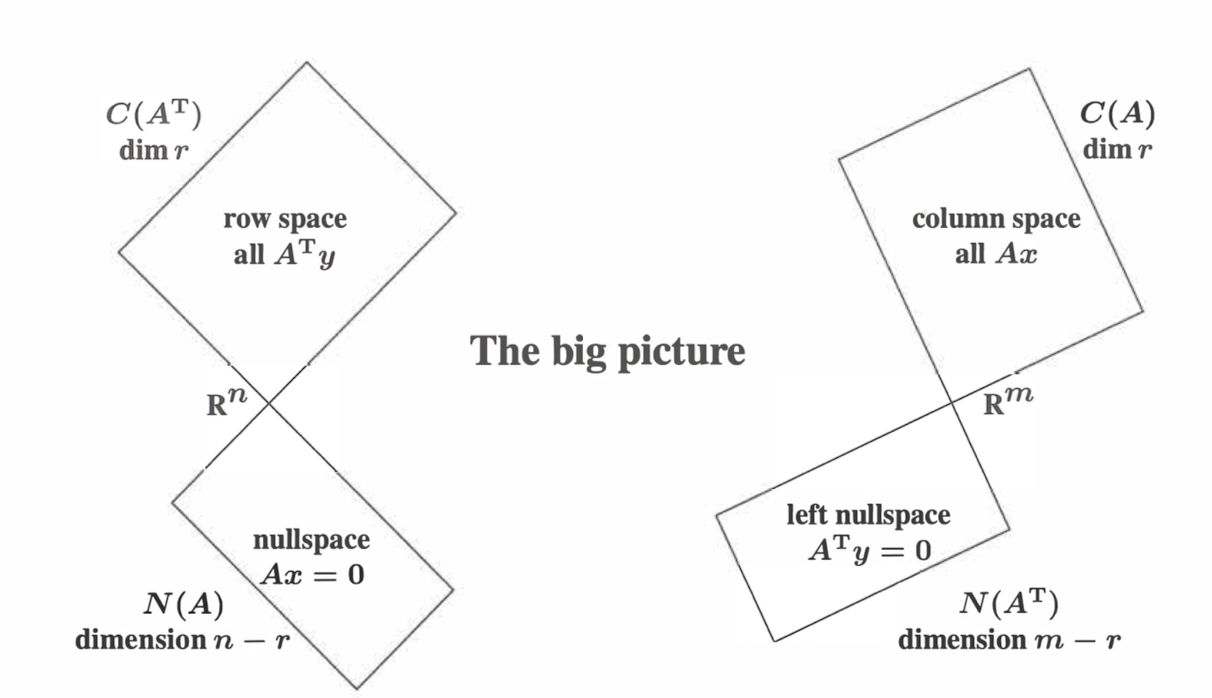
\includegraphics[width=0.7\linewidth]{../img/screenshot001}
	\caption{四个空间之间的相互关系}
	\label{image_big_picture}
\end{figure}


\subsection{正交性}

对于两个向量而言
$$
\begin{aligned}
	\mathbf u =\begin{bmatrix}1\\-1\end{bmatrix}\quad&\mathbf v=\begin{bmatrix}-1\\1\end{bmatrix}\\
	\mathbf u^\top\mathbf v&=\mathbf 0
\end{aligned}
$$
利用矩阵乘法的性质,我们可以用 $\mathbf u^\top\mathbf v$ 表示两个向量的点乘,点乘的值为 $0$ 那么两个向量就正交。


如果是两个矩阵正交:可以采用同样的定义 $\mathbf A^\top\mathbf B=\mathbf 0$ 。

线性代数的理论部分大致就到此结束。

\section{行列式}

很多线性代数开篇就是介绍行列式的计算,但行列式本身的意义其实必须要在能够理解向量空间后能够理解。所以本文将行列式的介绍放在了一个较后的位置。

对于一个 $n\times n$ 的矩阵,行列式的几何含义是:

\begin{quote}
	定义在n维空间下一组单位正交基所构成的体积为1。
	
	一个矩阵的行列式就等于,这个n维矩阵的列(或行)向量组所张成的体积。
\end{quote}

我们看一个非常简单的例子,如果是一个 $3\times 3$ 的矩阵:
$$
\begin{bmatrix}1 & 0 & 0\\0 & 2 & 0\\0 & 0 &1\end{bmatrix}
$$
这一组列向量显然是将y轴拉伸了2倍,张成的体积就是标准单位正交基张成空间的两倍。自然其行列式的值就是2。

现实中的向量组不会像这里的都是正交的,遇到非正交的向量组很难再通过求解体积的方式来计算行列式,所以你还是需要掌握行列式的求解方法。

通过这个定义,你就可以明白,为什么必须是方阵才能计算行列式,为什么不满秩的方阵其行列式一定为0(两个问题都请读者思考一下)。




